\documentclass{unswmaths}
\usepackage{shortcuts}
\usepackage[all]{xy}
\usepackage{csquotes}
\usepackage{color}
\usepackage[square,numbers]{natbib}
\usepackage{tikz}
\usepackage{pdfpages}

\begin{document}

\subject{Graph Theory}
\author{Ed McDonald}
\title{Assignment 2}
\studentno{z3375335}


\setlength\parindent{0pt}


\unswtitle{}

\includepdf[pages={1}]{cover_sheet.pdf}

\section*{Question 1}
For graphs $G$ and $H$, we let consider the graph
product $G\times H$ as having the vertex set $V(G)\times V(H)$,
and we have an edge $(v,w)(v',w') \in E(G\times H)$
if and only if $v = v'$ and $ww' \in E(H)$ or $vv' \in E(G)$ and $w = w'$. 

For a graph $G$, $\alpha(G)$ denotes the size of the largest independent
set in $G$.

\begin{lemma}[Part (a)]
    Let $G$ be a graph on $n \geq 2$ vertices, and let $r \geq 1$. Then
    \begin{equation*}
        \alpha(G \times K_r) \leq n.
    \end{equation*}     
\end{lemma}
\begin{proof}
    It is sufficient to show that any set of $n+1$ vertices
    in $G\times K_r$ has an adjacent pair. 
    Let $(v_1,w_1),(v_2,w_2),\ldots,(v_{n+1},w_{n+1}) \in V(G\times K_r)$,
    where each $v_k \in G$ and each $w_k \in K_r$. 
    
    By the pigeonhole principle, not all the $v_k$ can be distinct,
    so we must have $v_k = v_j$ for some $j \neq k$. Now since
    $K_r$ is complete, $w_kw_j \in E(K_r)$. Hence, $(v_k,w_k)(v_j,w_j) \in E(G\times K_r)$,
    so any set of $n+1$ vertices must have an adjacent pair.
    
    Hence, $\alpha(G\times K_r) \leq n$.    
\end{proof}

\begin{lemma}[Part (b)]
\label{1b}
    For a graph $G$ on $n \geq 2$ vertices, and $r \geq 1$, we have
    $\alpha(G\times K_r) = n$ if if $r = \chi(G)$.
\end{lemma}
\begin{proof}
    Let $r = \chi(G)$. We must show that $\alpha(G\times K_r)$
    has an independent set of size $n$. Choose an $r$-colouring
    for $G$, $c:G\to \{1,2,\ldots,r\}$. Let $V_j = c^{-1}(\{j\})$
    be the set of vertices of $G$ with colour $j$.
       
    Label the vertices of $K_r$ as $w_1,w_2,\ldots, w_r$. 
    
    Consider the set of vertices $S = \{(v,w_j)\;v \in V_j, 0 \leq j \leq r\}$.
    We shall show that $S$ is an independent set. Let $(v,w_j), (v',w_k) \in S$. 
    Then the vertices $(v,w_j),(v',w_k)$ are adjacent if and only if one of
    two possibilities holds:
    
    Firstly, if $w_j = w_k$, then $(v,w_j),(v',w_k)$ are adjacent
    if and only if $vv' \in E(G)$. But this is impossible since $v,v' \in V_j$.
    So $v$ and $v'$ both have colour $j$ so cannot be adjacent.
    
    The second case is that $j \neq k$, but we have $v = v'$. But then
    $v$ has colour $j$, and $v'$ has colour $k$. But this is impossible
    since $v = v'$.
    
    Thus, the vertices $(v,w_j),(v',w_k)$ are never adjacent.
    
    Now, the size of $S$ is just $|S| \sum_{j = 1}^r |\{(v,w_j)\;:\;v \in V_j\}| = \sum_{j=1}^r |V_j| = |V(G)|$,
    since the colour clases form a partition of $G$.
    
    Hence, $|S| = n$, so we have an independent set of size $n$.    
\end{proof}

\begin{corollary}[Part (c)]
    For a graph $G$ on $n\geq 2$ vertices, we have:
    \begin{equation*}
        \chi(G) = \min\{r > 0\;:\;\alpha(G\times K_r) = n\}.
    \end{equation*}
\end{corollary}
\begin{proof}
    By lemma \ref{1b}, we know that $\alpha(G\times K_r) = n$
    when $r = \chi(G)$. We must show that $\alpha(G \times K_r) < n$
    when $r < \chi(G)$. 
    
    We will show this by demonstrating how an independent
    set of size $n$ in $G \times K_r$ induces a colouring
    of $G$ with at most $r$ colours. Since this is possible only when $r \geq \chi(G)$,
    this will prove that there are no independent sets
    of size $n$ in $G\times K_r$ when $r < \chi(G)$.
    
    Let $r \geq 1$, and suppose that $S$ is an independent
    set of size $n$ in $G\times K_r$, and label
    the vertices of $K_r$ as $w_1,w_2,\ldots,w_r$.
    
    First we show that for all $v \in V$, there
    is some $j$ so that $(v,w_j) \in S$. 
    If this is not the case, then by the pigeonhole principle
    there must be some $v \in V$ such that $(v,w),(v,u) \in S$
    for distinct $w,u \in K_r$. But then $wu \in E(K_r)$, so $(v,w)$
    and $(v,u)$ are adjacent, which is impossible
    since $S$ is independent.
    
    Now we can define a function $c:V(G)\to \{1,2,\ldots,r\}$
    as follows. 
    
    We define $c(v) = j$ if $(v,w_j) \in S$. 
    This is well defined, since if $(v,w_j),(v,w_k) \in S$
    are distinct, we must have that $w_j w_k \in E(K_r)$.
    Hence $c(v)$ is defined uniquely for at least some vertices
    in $G$.
    
    In fact $c$ is a colouring of $G$. To see this, let $vv' \in E(G)$. 
    If $c(v) = c(v') = j$, then $(v,w_j),(v',w_j) \in S$.
    But then since $v$ and $v'$ are adjacent, we must have that $(v,w_j)$
    and $(v',w_j)$ are adjacent. Since $S$ is independent, we must then
    have $c(v) \neq c(v')$. 
    
    Hence $c$ is a colouring of $v$ with at most $r$ colours,
    and we are done.    
\end{proof} 

\section*{Question 2}
For this question, $G$ is a $3$-connected graph and $xy \in E(G)$. 
We use the notation $G/xy$ to denote the graph obtained from $G$
by contracting $xy$.

\begin{proposition}[Part (a)]
    If $G/xy$ is $3$-connected, then $G - \{x,y\}$ is $2$-connected.
\end{proposition}
\begin{proof}
    To show that $G-\{x,y\}$ is $2$-connected, at the very least it must have at
    least three vertices. To show this, we note that by assumption $G/xy$ is $3$-connected,
    and $|V(G/xy)| = |V(G)|-1$. Since $G/xy$ is itself $3$-connected, we have $|V(G/xy)| > 3$.
    Hence, $|V(G)| > 4$. Thus, $|V(G-\{x,y\})| > 2$. 
    
    Now we need to show that $G-\{x,y\}$ is connected, and for any vertex $v \in V(G-\{x,y\})$,
    $G-\{x,y,v\}$ is connected. 
    
    Now since $G$ is by assumption $3$-connected, automatically we have that $G-\{x,y\}$ is connected.
    Hence it is only required to show that $G-\{x,y,v\}$ is connected for all
    vertices $v \in V(G-\{x,y\})$. 
    
    So let $v \in V(G-\{x,y\})$. Hence $v \in V(G/xy)$.
    Let $w$ be the vertex in $G/xy$ formed from merging $x$ and $y$.
    
    Thus, $G/xy-\{v,w\}$ is connected since $G/xy$ is $3$-connected by assumption.
    
    Let $p,q \in V(G-\{x,y,v\})$. Since $G/xy-\{v,w\}$ is connected,
    there is a path $P$ joining $p$ and $q$ in $G/xy$ which avoids $v$ and $w$. 
    
    Hence every edge of $P$ consists of edges of $G/xy-\{v,w\}$. 
    Since every edge of $G/xy-\{v,w\}$ is an edge of $G$, $P$
    can be considered as a path in $G$. Since it avoids $v$ and $w$, it 
    must avoid $x,y$ and $v$ in $G$.     
    
    Thus $G-\{x,y,v\}$ is
    connected, and so $G-\{x,y\}$ is connected. 
\end{proof}

\begin{proposition}[Part (b)]
    Now if $G/xy$ is \emph{not} $3$-connected, then $G-\{x,y\}$ is not
    $2$-connected.
\end{proposition}
\begin{proof}
    We shall prove the contrapositive. Suppose that $G-\{x,y\}$
    is $2$-connected. In particular, this means that $G-\{x,y\}$
    has at least three vertices, so $G$ has at least five vertices.
    Hence, $G/xy$ has at least four vertices. 
    
    Now to complete the proof we need to show that removing any $2$ element
    subset of $G/xy$ does not disconnect $G/xy$. 
    
    Now by assumption, $G-\{x,y\}$ is $2$-connected. In particular
    this means that it is connected, and for any $v \in V(G)-\{x,y\}$
    we have that $G-\{x,y,v\}$ is connected.
    
    Now, let $u,w \in V(G/xy)$. Then there are two possibilities:
    \begin{enumerate}
        \item{} One of $u$ or $v$ is formed by contracting $x$ and $y$.
        \item{} Neither of $u$ and $v$ is formed by contracting $x$ and $y$.
    \end{enumerate}
    In the first case, we may assume without loss of generality that $u$
    is formed from contracting $x$ and $y$. We now
    consider $G/xy-\{u,w\}$. This is simply $G-\{x,y,w\}$. But by assumption
    this is connected, hence $G/xy-\{u,w\}$ is connected.
    
    In the second case, we have $u,v \in V(G-\{x,y\})$. Now, let $H = G/xy-\{u,v\}$.
    
    Now, let $p,q \in V(H)$. We must show that there is a path joining $p$ and $q$
    in $H$. Since neither $u$ nor $v$
    is formed from contracting $x$ and $y$, it is sufficient to show that there is a path joining $p$
    and $q$ in $G$ which avoids $u$ and $v$. Hence, we search for a path
    in $G-\{u,v\}$. However, by assumption $G$ is $3$-connected, so such a path exists.
    Hence, $H$ is connected. 
    
    Thus, $G/xy$ is $3$-connected, as required.
\end{proof}

\section*{Question 3}
For this question, $G$ is a graph and $P_G(k)$ denotes
the number of $k$-colourings of $G$. It is known that $P_G(k)$
is polynomial in $k$, and is hence called the chromatic polynomial of $G$.

From the problem sheets, we know that if $G$ has $n$ vertices then $P_G(k)$
is a monic polynomial of degree $n$, and if $G$ has $m$ edges 
then the coefficient of $k^{n-1}$ is $-m$.

Since this is not proved in the notes, we give a short proof here. 
Let $x,y \in V(G)$, and let $G' = G-xy$ and $G''$ be the graph
obtained by contracting $x$ and $y$. 
Now a $k$-colouring of $G$ is exactly a $k$-colouring
of $G'$ which assigns different colours to $x$ and $y$. 
The $k$-colourings of $G$ which assign the same colours to $x$ and $y$
are exactly the $k$-colourings of $G''$. Hence, $P_G(k) = P_{G'}(k)-P_{G''}(k)$. 
Hence if we do induction on the number of edges of $G$, we can prove the
required properties of $P_G(k)$.

\begin{lemma}[Part (a)]
    There is no graph $G$ with chromatic polynomial
    \begin{equation*}
        P_G(k) = k^4-4k^3+8k^2-5k.
    \end{equation*}
\end{lemma}
\begin{proof}
    Let $G$ be such a graph. Then $G$ must have $4$
    vertices and $4$ edges. Hence, by the handshaking
    lemma the average degree of $G$ is $2$. Hence $G$ is $2$-regular
    or has a vertex of degree $3$.
    
    If $G$ is $2$-regular, then $G = C_4$ is a cyclic graph on $4$ vertices.
    Hence, in this case, the number of $2$-colourings of $G$ is $2$.
    
    However $P_G(2) = 16-32+32-10 = 6$, so $G \neq C_4$.
    
    The only other case is that $G$ has a vertex of degree $3$. 
    Since $|V(G)| = 4$, this means that $G$ has a vertex $v$, connected to every 
    other vertex. Hence if we have a $2$-colouring of $G$, $c:V(G)\to \{1,2\}$
    we either have $c(v) = 1$ and all other vertices have colour $2$,
    or $c(v) = 2$ and all other vertices have colour $1$.
    However this cannot be a true colouring since there are four edges: so one
    edge must connect two vertices of colour $2$. Hence there is no $2$-colouring
    of $G$. Thus, $p_G(k) = 0 \neq 6$.
    
    Thus we have exhausted all possible graphs with four vertices and four
    edges. Hence the given polynomial cannot be a chromatic polynomial.
\end{proof}

\begin{lemma}[Part (b)]
\label{3b}
    Let $G$ be a graph, with $v \in V(G)$. Then the number of $k$-colourings
    of $G$ which assign colour $1$ to $v$ is given by $P_G(k)/k$.
\end{lemma}
\begin{proof}
    Let $C_i$ be the number of colourings which assign colour $i$ to $v$. 
    Then, 
    \begin{equation*}
        P_G(k) = C_1+C_2+\cdots+C_k.
    \end{equation*}
    Now by symmetry, we have $C_1 = C_i$ for all $i$, hence,
    \begin{equation*}
        P_G(k) = kC_1
    \end{equation*}
    as required.
\end{proof}

\begin{lemma}[Part (c)]
\label{3c}
    Let $G$ be a graph with connected components $G_1,G_2,\ldots,G_r$.
    Then 
    \begin{equation*}
        P_G(k) = \prod_{j=1}^r P_{G_j}(k).
    \end{equation*}
\end{lemma}
\begin{proof}
    Let $k \geq 1$. Then for each $1 \leq j \leq r$, a $k$-colouring
    of $G$ induces a $k$-colouring of $G_j$. Thus each $k$-colouring
    of $G$ is produced by an individual $k$ colouring of each $G_j$. 
    Hence, the number of $k$-colourings of $G$ is given by a $k$-colouring
    of $G_1$, times the number of $k$-colourings of $G_2$, times 
    the number of $k$-colourings of $G_2$, and etc., until we have
    a $k$-colouring for $G$.
\end{proof}

\begin{lemma}[Part (d)]
    Let $r > 0$ and let $G$ have $r$ connected components. If:
    \begin{equation*}
        P_G(k) = c_0 + c_1k+c_2k^2 + \cdots + c_nk^n
    \end{equation*}
    we have $c_0 = c_1 = \ldots = c_{r-1} = 0$
    and $c_r \neq 0$.
    
    In other words, if $G$ has $r$ connected components, then
    $r$ is the minimal positive integer such that the coefficient
    of $k^r$ in $P_G(k)$ is nonzero.
   
    Alternatively, $k$ divides $P_G(k)$ at least $r$ times.
    
\end{lemma}
\begin{proof}
%    First we prove the case where $r = 1$. That is,
%    we wish to prove that if $G$ is a connected graph, then $k$ divides $P_G(k)$
%    exactly once. 
%    
%    Let $v \in V(G)$.
%    Now if $G$ is connected, the number of $k$-colourings of $G$
%    which give vertex $v$ colour $1$ must be \emph{strictly less} than the number
%    of $k$-colourings of $G-v$. The strictness comes from the fact
%    that $v$ has a neighbour, and hence this neighbour can be colours with
%    colour $1$.
%    Thus, by lemma \ref{3b},
%    \begin{equation}
%    \label{ineq}
%        \frac{P_G(k)}{k} < P_{G-v}(k)
%    \end{equation}
%    for all $k \geq 2$. 
%    
%    We now prove that $P_G(k)$ has exactly one factor of $k$ by induction
%    on $n = V(G)$.
%    
%    For the case $n = 1$, $G$ is a single vertex, so $P_G(k) = k$,
%    so the result holds for $n = 1$. 
%    
%    Now suppose that the result holds for $n \geq 1$, and suppose that $G$ has $n+1$
%    vertices.
    
%    Since $G$ is connected, there exists some $v \in V(G)$ such
%    that $G-v$ remains connected (we can see this by letting $v$ be a leaf
%    of a spanning tree of $G$).
%    
%    Hence by the inductive hypothesis, $k$ divides $P_{G-v}(k)$ exactly once,
%    so $P_{G-v}'(0) \neq 0$. 
%    Since $G-v$ is connected, $P_{G-v}(1) = 0$. 
%    
%    
    Let the connected components of $G$ be $\{G_i\}_{i=1}^r$. Then
    by lemma \ref{3c}, we have:
    \begin{equation*}
        P_G(k) = \prod_{i=1}^r P_{G_i}(k).
    \end{equation*}
    By lemma \ref{3b}, $k$ divides $P_{G_i}(k)$.
    Hence, $k$ divides $P_G(k)$ at least $r$ times.
\end{proof}

Now for Part (e), the following graph has chromatic polynomial
$P_G(k) = k^2(k-1)^3(k-2)$:
\begin{center}
    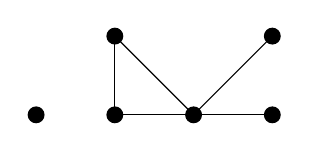
\begin{tikzpicture}
        \draw [fill] (0,0) circle (0.1);
        \draw [fill] (1,0) circle (0.1);
        \draw [fill] (1,1) circle (0.1);
        \draw [fill] (2,0) circle (0.1);
        \draw [fill] (3,0) circle (0.1);
        \draw [fill] (3,1) circle (0.1);
        
        \draw [-] (1,0) -- (1,1);
        \draw [-] (1,0) -- (2,0);
        \draw [-] (1,1) -- (2,0);
        \draw [-] (2,0) -- (3,0);
        \draw [-] (2,0) -- (3,1);
    \end{tikzpicture}
\end{center}

\section*{Question 4}
For this question, $k \geq 1$ and $G = (V,E)$ is a $k$-edge connected
graph. We let $F_1,\ldots,F_m \subseteq E$ be distinct sets of $k$ edges
which disconnected $G$. We let $\mathcal{F} = F_1\cup F_2\ldots \cup F_m$,
and let $C_1,\ldots,C_t$ be the connected components of $G-\mathcal{F}$.

\begin{lemma}[Part (a)]
\label{4a}
    For each $i = 1,\ldots,m$, we have:
    \begin{equation*}
        |\{e \in \mathcal{F}\;:\;e \cap C_i \neq \emptyset\}| \geq k.
    \end{equation*}
\end{lemma}
\begin{proof}
    Since $G$ is $k$-connected, it suffices to show that $S_i = \{e \in \mathcal{F}\;:\;e \cap C_i \neq \emptyset\}$
    disconnects $G$. 
    
    Consider $G-S_i$. Suppose that $e$ is an edge joining $C_i$ to $G-C_i$. Then
    since $C_i$ is a connected component of $G-\mathcal{F}$, we must have $e \in \mathcal{F}$,
    and in particular $e \in S_i$. Hence $e \notin G-S_i$, so $G-S_i$
    contains no edges joining $C_i$ to $G-C_i$. Thus $G-S_i$ is disconnected, 
    and hence $|S_i| \geq k$.
\end{proof}

\begin{corollary}[Part (b)]
    We have $|\mathcal{F}| \geq kt/2$.
\end{corollary}
\begin{proof}
    Now, each $e \in \mathcal{F}$ is incident with at least one $C_i$, and at
    most two $C_i$. Let $S_i$ as in lemma \ref{4a}, and we have:
    \begin{equation*}
        \mathcal{F} = S_1\cup S_2\cup \ldots \cup S_t. 
    \end{equation*}
    However, each element of $\mathcal{F}$ occurs in at most two of the $S_i$. 
    Thus the sum
    \begin{equation*}
       \sum_{i=1}^t |S_i|
    \end{equation*}
    counts each element of $\mathcal{F}$ at most twice. Hence,
    \begin{equation*}
        \sum_{i=1}^t |S_i| \leq 2|\mathcal{F}|.
    \end{equation*}
    Hence, since for each $i$ we have $|S_i| \geq k$ from lemma \ref{4a}, 
    \begin{equation*}
        kt \leq 2|\mathcal{F}|.
    \end{equation*}
    So the result follows.
\end{proof}

\begin{corollary}[Part (c)]
    We have $|\mathcal{F}| \leq mk$, and hence $t \leq 2m$.
\end{corollary}
\begin{proof}
    Since $\mathcal{F} = F_1\cup F_2\cup\cdots\cup F_m$, hence $|\mathcal{F}| \leq |F_1|+|F_2|+\cdots+|F_m|$. 
    Since each $|F_i| = k$, we then have $|\mathcal{F}| \leq mk$. 
    Thus,
    \begin{equation*}
        kt/2 \leq |\mathcal{F}| \leq mk.
    \end{equation*}
    and hence $t \leq 2m$. 
\end{proof}


\section*{Question 5}

For this question, $H$ denotes a $3$-uniform hypergraph
on $n$ vertices with $n$ element vertex set $V$
and $m$ element hyperedge set $E$, and $m \geq n/3$.

\begin{lemma}[Part (a)]
    \label{5a}
    Let $U \subset V$ be a random vertex set, with $v \in U$
    with probability $p$. Then $\mathbb{E}(|U|) = np$.
\end{lemma}
\begin{proof}
    Let $X:G\to \{0,1\}$ be the indicator function of the set $U$.
    Then by the linearity of expectation,
    \begin{equation*}
        \mathbb{E}(|U|) = \sum_{v \in V} \mathbb{E}(X(v)).
    \end{equation*}
    Now, $X(v) = 1$ with probability $p$ and $0$ with probability $1-p$.
    Hence $\mathbb{E}(X(v)) = p$, so $\mathbb{E}(|U|) = np$.
\end{proof}

\begin{lemma}[Part (b)]
\label{5b}
    Define $Y$ to be the number of hyperedges contained in $U$, randomly
    chosen as in lemma \ref{5a}, that is,
    \begin{equation}
        Y = |\{e \in E\;:\;e \subseteq U\}|.
    \end{equation}
    Then $\mathbb{E}(Y) = mp^3$.
\end{lemma}
\begin{proof}
    Let $X:E\to \{0,1\}$ be the indicator function
    of the set of hyperedges in $U$.
    Then by the linearity of expectation,
    \begin{equation*}
        \mathbb{E}(Y) = \sum_{e \in E} \mathbb{E}(X(e)).
    \end{equation*}
    So we need to compute $\mathbb{E}(X(e))$ for a given
    hyperedge $e$. 
    
    Since $X(e) = 1$ if $e \subseteq U$, and $0$ otherwise,
    we have that $\mathbb{E}(X(e))$ equal the probability
    that $e \subseteq U$. In otherwords, $\mathbb{E}(X(e))$
    is the probability that $U$ contains $e$. 
     
    Suppose that $e = \{u,v,w\}$. Then $\mathbb{E}(X(e)) = \mathbb{P}(u,v,w \in U)$. 
    Since each vertex is chosen to be in $U$ with probability $p$ independently,
    we have that $\mathbb{E}(X(e)) = p^3$. 
    Thus,
    \begin{align*}
        \mathbb{E}(Y) &= \sum_{e \in E} p^3\\
                      &= mp^3.
    \end{align*}
\end{proof}

\begin{corollary}[Part (c)]
\label{5c}
    Hence, $H$ contains an independent set with at least $\frac{2n^{3/2}}{3\sqrt{3m}}$
    vertices.
\end{corollary}
\begin{proof}
    We will use the probabilistic method: we will define
    a random independent subset of $H$ and show that the
    expected value of its size is at least $\frac{2n^{3/2}}{3\sqrt{3m}}$.
    
    Let $U \subseteq H$ be chosen as in lemma \ref{5a}, and let
    $Y$ be the number of edges in $U$ as in lemma \ref{5b}. 
    
    If we remove one vertex from every edge in $U$, then we create an independent
    set. Hence we can remove $Y$ vertices from $H$ to form an independent set
    of size $|U|-Y$.
    By the linearity of expectation, and lemmas \ref{5a} and \ref{5b}:
    \begin{align*}
        \mathbb{E}(|U|-Y) &= \mathbb{E}(|U|)-\mathbb{E}(Y)\\
                          &= np - mp^3.
    \end{align*}
    Hence there exists an independent set of size at least $np-mp^3$. 
    
    Since this holds for all $p \in [0,1]$, we can choose $p$ freely
    in this range.
    Let $p = \sqrt{n/3m}$. This is a true probability
    since by assumption $m \geq n/3$. Then,
    \begin{align*}
        np - mp^3 &= \sqrt{\frac{n}{3m}}(n-m\frac{n}{3m})\\
                  &= \frac{2n^{3/2}}{3\sqrt{3m}}.
    \end{align*}
    Hence there is an independent set of at least this size.
\end{proof}

\begin{remark}
    Our choice for $p$ in the proof of corollary \ref{5c} in fact
    maximises $np-mp^3$ for $p \in [0,1]$, but it is not necessary to show this since we only
    require a lower bound.
\end{remark}

\end{document}
